\section{Architecture}
\subsection{Data formats}
\label{subsec:data-formats}

The \textit{structured document} contains three main sections: a) bibliographic data (authors, DOI, title, publisher, journal, year of publication), b) runtime execution time from the server side (excluding the network and database delay), and c) a list of text passages, each representing a sentence.
Each passage is then composed of the following attributes (Figure~\ref{fig:data-flow-2} (orange): 
\begin{itemize}
\item the text of the passage
\item the type of passage: sentence, or paragraph
\item the main section: body, header, or annex
\item the subsection within the section: title, abstract, paragraph, caption, etc.
\item the list of spans where each span represents one entity extracted from the text (Figure~\ref{fig:data-flow-2} (orange)).
\item a list of layout tokens: layout information such as font size, font name, superscript, subscript, bold, and italic taken from the PDF document.
\end{itemize}

\begin{figure}[htbp]
  \centering
  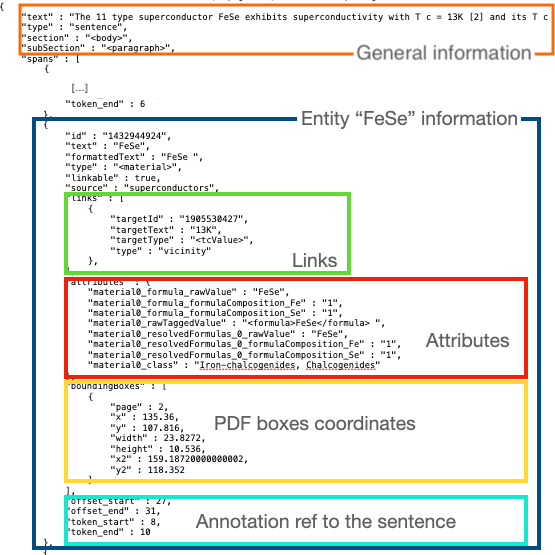
\includegraphics[width=1\textwidth]{images/data-flow-2} 
  \caption{Example of span encoding information of a passage (orange) with focus on the extracted material \textit{FeSe} (blue). 
  The links (green) indicate linked entities and their type (in our example the material FeSe is linked to 13K of type \texttt{<tcValue>}. 
  The attributes (red) are key-value information extracted or aggregated by external tools (e.g. Material Parser or class identifier module described in \cite{lfoppiano2023automatic}).
  The "PDF boxes coordinates" (yellow) is a list of coordinates in respect of the PDF document. 
  Finally, the "Annotation references" (light blue) position the span within the sentence by character count or token counts.}
  \label{fig:data-flow-2}
\end{figure}

Each span aggregates a complex set of information illustrated in an example in Figure~\ref{fig:data-flow-2} (blue): links (in green), attributes (in red), PDF "boxes" coordinates (in yellow), and annotation reference to the sentence (in light blue). 
The "PDF boxes coordinates" (yellow) are information to draw a set of rectangles on the PDF document ("the boxes") that encapsulate groups of tokens belonging to each annotation\footnote{Details on coordinates is available in the official grobid documentation \url{https://grobid.readthedocs.io/en/latest/Coordinates-in-PDF/\#coordinates-in-teixml-results}}.

The "Aggregation Task" transforms the "structured document" in input to a tabular format comprising as many rows as the extracted materials records. The format is described in detail in \cite{lfoppiano2023automatic}.

\section{Evaluation}
\label{app:interface-evaluation-raw}
\subsection{Interface evaluation}

\begin{table}[h]
\centering
\small
\caption{Timetable recording the time spent for each of the 15 articles. Each row indicates the time and the event (Starting, Finishing) from each of the curators: Master Student (MD), PhD Student (PD), and Senior Researcher (SD).}
\begin{tabular}{cc|cc|c}
Time & Event & Document ID & Curator & Duration (mins) \\
\hline
14:40 & Start   & 02bf1b3db9 & PS  & 0  \\
14:49 & Finish  & 02bf1b3db9 & PS  & 9  \\
14:53 & Start   & 00b50fc0a8 & PS  & 0  \\
14:58 & Finish  & 00b50fc0a8 & PS  & 5  \\
14:37 & Start   & 0aa1b3161f & MS  & 0  \\
14:50 & Start   & 0454e07f64 & SR  & 0  \\
14:58 & Finish  & 0454e07f64 & SR  & 8  \\
15:01 & Start   & 02cbc58819 & PS  & 0  \\
15:06 & Start   & 00c32076f4 & SR  & 0  \\
15:07 & Finish  & 0aa1b3161f & MS  & 30 \\
15:08 & Finish  & 02cbc58819 & PS  & 7  \\
15:08 & Start   & 044939701d & PS  & 0  \\
15:12 & Start   & 0021fd339f & MS  & 0  \\
15:15 & Finish  & 00c32076f4 & SR  & 9  \\
15:17 & Finish  & 044939701d & PS  & 9  \\
15:17 & Start   & 08e1cb8f4f & PS  & 0  \\
15:20 & Start   & 0c7d3163ea & SR  & 0  \\
15:31 & Finish  & 08e1cb8f4f & PS  & 14 \\
15:32 & Finish  & 0021fd339f & MS  & 20 \\
15:32 & Start   & 039105663f & MS  & 0  \\
15:37 & Finish  & 0c7d3163ea & SR  & 17 \\
15:53 & Finish  & 039105663f & MS  & 21 \\
15:55 & Start   & 02c4f00127 & MS  & 0  \\
15:58 & Start   & 0454e07f64 & PS  & 0  \\
16:02 & Start   & 0da5febabf & SR  & 0  \\
16:08 & Finish  & 0454e07f64 & PS  & 10 \\
16:09 & Finish  & 02c4f00127 & MS  & 14 \\
16:11 & Finish  & 0da5febabf & SR  & 9  \\
16:11 & Start   & 0012333581 & SR  & 0  \\
16:12 & Start   & 00c32076f4 & PS  & 0  \\
16:18 & Start   & 021c413172 & MS  & 0  \\
16:22 & Finish  & 00c32076f4 & PS  & 10 \\
16:23 & Start   & 0c7d3163ea & PS  & 0  \\
16:30 & Finish  & 0012333581 & SR  & 19 \\
16:32 & Finish  & 021c413172 & MS  & 14 \\
16:37 & Start   & 02bf1b3db9 & MS  & 0  \\
16:38 & Finish  & 0c7d3163ea & PS  & 15 \\
17:32 & Finish  & 0021fd339f & SR  & 12 \\
17:34 & Start   & 039105663f & SR  & 0  \\
17:55 & Finish  & 039105663f & SR  & 21 \\
17:56 & Start   & 02c4f00127 & SR  & 0  \\
18:00 & Finish  & 02c4f00127 & SR  & 4  \\
18:00 & Start   & 021c413172 & SR  & 0  \\
18:09 & Finish  & 021c413172 & SR  & 9  \\
\end{tabular}
\end{table}


\begin{table}[h]
\centering
\small
\caption{Detailed evaluation metrics for each combination of article, method and curator. }
\begin{tabular}{cc|c|ccc|ccc}

Document ID & \# pages & Method & \# TP	& \# FP	& \# FN	& P	& R	& F1 \\
\hline
0454e07f64  & 4     & I     & 6     & 0     &   0   & 100.00    & 100.00    & 100.00 \\
00c32076f4  & 13    & P     & 8     & 0     &   0   & 100.00    & 100.00    & 100.00 \\
0c7d3163ea  & 9     & I     & 13    & 1     &   0   & 92.86     & 100.00    & 96.30 \\
0da5febabf  & 11    & P     & 8     & 0     &   1   & 100.00    & 88.89     & 94.12 \\
0012333581  & 13    & I     & 11    & 0     &   0   & 100.00    & 100.00    & 100.00 \\
0aa1b3161f  & 5     & I     & 9     & 0     &   1   & 100.00    & 90.00     & 94.74 \\
0021fd339f  & 14    & P     & 4     & 0     &   8   & 100.00    & 33.33     & 50.00 \\
039105663f  & 9     & I     & 11    & 1     &   0   & 91.67     & 100.00    & 95.65 \\
02c4f00127  & 13    & P     & 0     & 0     &   3   & 100.00    & 0.00      & 0.00 \\
021c413172  & 5     & I     & 15    & 0     &   0   & 100.00    & 100.00    & 100.00 \\
0aa1b3161f  & 5     & P     & 1     & 0     &   9   & 100.00    & 10.00     & 18.18 \\
0021fd339f  & 14    & I     & 12    & 3     &   3   & 80.00     & 100.00    & 88.89 \\
039105663f  & 9     & P     & 4     & 1     &   7   & 80.00     & 41.67     & 54.79 \\
02c4f00127  & 13    & I     & 3     & 1     &   1   & 75.00     & 100.00    & 85.71 \\
021c413172  & 5     & P     & 7     & 1     &   7   & 87.50     & 53.33     & 66.27 \\
02bf1b3db9  & 7     & P     & 2     & 0     &   5   & 100.00    & 28.57     & 44.44 \\
00b50fc0a8  & 11    & I     & 7     & 2     &   0   & 77.78     & 100.00    & 87.50 \\
02cbc58819  & 4     & P     & 5     & 0     &   2   & 100.00    & 71.43     & 83.33 \\
044939701d  & 12    & I     & 5     & 0     &   1   & 100.00    & 83.33     & 90.91 \\
08e1cb8f4f  & 16    & P     & 1     & 0     &   6   & 100.00    & 14.29     & 25.00 \\
02bf1b3db9  & 7     & I     & 5     & 0     &   2   & 100.00    & 71.43     & 83.33 \\
00b50fc0a8  & 11    & P     & 2     & 0     &   7   & 100.00    & 22.22     & 36.36 \\
02cbc58819  & 4     & I     & 4     & 0     &   3   & 100.00    & 57.14     & 72.73 \\
044939701d  & 12    & P     & 4     & 0     &   2   & 100.00    & 66.67     & 80.00 \\
08e1cb8f4f  & 16    & I     & 5     & 1     &   1   & 83.33     & 85.71     & 84.51 \\
0454e07f64  & 4     & P     & 0     & 1     &   5   & 0.00      & 16.67     & 0.00 \\
00c32076f4  & 13    & I     & 8     & 0     &   0   & 100.00    & 100.00    & 100.00 \\
0c7d3163ea  & 9     & P     & 9     & 0     &   5   & 100.00    & 64.29     & 78.26 \\
0da5febabf  & 11    & I     & 9     & 0     &   0   & 100.00    & 100.00    & 100.00 \\
0012333581  & 13    & P     & 4     & 4     &   3   & 50.00     & 72.73     & 59.26 \\
\end{tabular}
\end{table}
